\documentclass[14pt,a4paper]{extarticle}
\usepackage{fontspec}
\defaultfontfeatures{Ligatures=TeX}
\usepackage{polyglossia}
\setdefaultlanguage{russian}
\setotherlanguage{english}
\IfFontExistsTF{Times New Roman}{\setmainfont{Times New Roman}}{\setmainfont{CMU Serif}}
\IfFontExistsTF{Times New Roman}{\newfontfamily\cyrillicfont{Times New Roman}}{\newfontfamily\cyrillicfont{CMU Serif}}
\setmonofont{lmmono10-regular.otf}[Scale=MatchLowercase]
\usepackage{amsmath,mathtools}
\usepackage{unicode-math}
\setmathfont{texgyretermes-math.otf}
\usepackage[left=27mm,right=20mm,top=20mm,bottom=22mm]{geometry}
\usepackage{graphicx,booktabs,array,tabularx,threeparttable,float,placeins}
\usepackage{caption,setspace,titlesec,titletoc,etoolbox}
\usepackage[hidelinks,unicode]{hyperref}
\usepackage{xurl}
\setstretch{1.20}
\setlength{\parindent}{1.25cm}
\setlength{\parskip}{0pt}
\setlength{\emergencystretch}{2em}
\raggedbottom
\clubpenalty=10000
\widowpenalty=10000
\brokenpenalty=10000
\displaywidowpenalty=10000
\pagestyle{plain}
\setcounter{tocdepth}{2}
\titleformat{\section}{\bfseries\large}{\thesection}{0.65em}{}
\titleformat{\subsection}{\bfseries\normalsize}{\thesubsection}{0.65em}{}
\titlespacing*{\section}{0pt}{1.2\baselineskip}{0.5\baselineskip}
\titlespacing*{\subsection}{0pt}{0.8\baselineskip}{0.35\baselineskip}
\titlecontents{section}[0em]{\addvspace{4pt}\bfseries}{\contentspush{\thecontentslabel\quad}}{}{\titlerule*[0.5pc]{.}\contentspage}
\titlecontents{subsection}[1.5em]{\small}{\contentspush{\thecontentslabel\quad}}{}{\titlerule*[0.5pc]{.}\contentspage}
\contentsmargin{2.5em}
\captionsetup{font=small,labelsep=period,justification=centering}
\captionsetup[table]{position=top,skip=6pt}
\setlength{\textfloatsep}{12pt}
\setlength{\intextsep}{12pt}
\newcommand{\PaperTableStyle}{\centering\small\setstretch{1}\setlength{\tabcolsep}{5pt}\renewcommand{\arraystretch}{1.15}}
\newcommand{\PaperTableNotesStyle}{\footnotesize\setstretch{1}}
\newcommand{\ReportStatus}[1]{\textbf{[#1]}}
\newcommand{\normE}[1]{\left\lVert #1\right\rVert_E}
\newcommand{\inner}[2]{\left(#1,#2\right)_h}
\newcommand{\mat}[1]{\mathbf{#1}}
\newcommand{\vect}[1]{\mathbf{#1}}
\newcommand{\code}[1]{\texttt{#1}}
\makeatletter
\newcommand{\DataInput}[1]{\@@input tables/#1.tex }
\makeatother
\AtBeginEnvironment{thebibliography}{\small\setstretch{1.1}}

\usepackage[autostyle=true]{csquotes}
\usepackage[backend=biber,style=numeric,sorting=none,giveninits=true,maxnames=5]{biblatex}
\addbibresource{references.bib}
\renewcommand*{\bibfont}{\small\setstretch{1.1}}

\hypersetup{pdftitle={Задача Дирихле для уравнения Пуассона. Вариант 14},pdfauthor={Глеб Костин}}
\begin{document}
\begin{titlepage}
    \centering
    \vspace*{0.4cm}
    
\includegraphics[width=6cm]{figures/university-000.png}\par
    \vspace{0.6cm}
    Московский государственный университет\\
    имени М. В. Ломоносова\par
    \vspace{2cm}
    {\Large Костин Глеб\par}
    \vspace{1.6cm}
    {\Large\bfseries Отчёт по практическому заданию № 1\par}
    \vspace{0.6cm}
    Суперкомпьютерное моделирование и технологии\par
    \vspace{1cm}
    Численное решение задачи Дирихле\\
    для уравнения Пуассона\par
    \vspace{0.5cm}
    Вариант 14\par
    \vfill
    Москва, 2026
\end{titlepage}
\setcounter{page}{2}

\tableofcontents
\clearpage
\section{Постановка задачи}

Рассматривается двумерная задача Дирихле для уравнения Пуассона.
Требуется найти функцию $u(x,y)$, которая удовлетворяет уравнению внутри заданной области и принимает известные значения на её границе:
\begin{equation}
    -\Delta u=1 \quad \text{в }
    D, \qquad u=\sin(x+y) \quad \text{на } \gamma=\partial D.
    \label{eq:problem}
\end{equation}
Здесь $\Delta u=\partial^2u/\partial x^2+\partial^2u/\partial y^2$ есть оператор Лапласа, $D$ обозначает область расчёта, а $\gamma$ её границу.
Координаты и значения функции в задании безразмерны.

Варианту 14 соответствует область~\cite{assignment}
\begin{equation}
    D=\left\{(x,y):x^2+(|y|-2)^2<9\right\}.
    \label{eq:domain}
\end{equation}
Она представляет собой объединение двух кругов радиуса $3$ с центрами $(0,2)$ и $(0,-2)$.
Для вычислений выбран прямоугольник $\Pi=(-4,4)\times(-6,6)$, внутри которого целиком находится замыкание $D$.
Форма области и пример её распределения между процессами показаны на рис.~\ref{fig:geometry}.

\begin{figure}[ht]
    \centering
    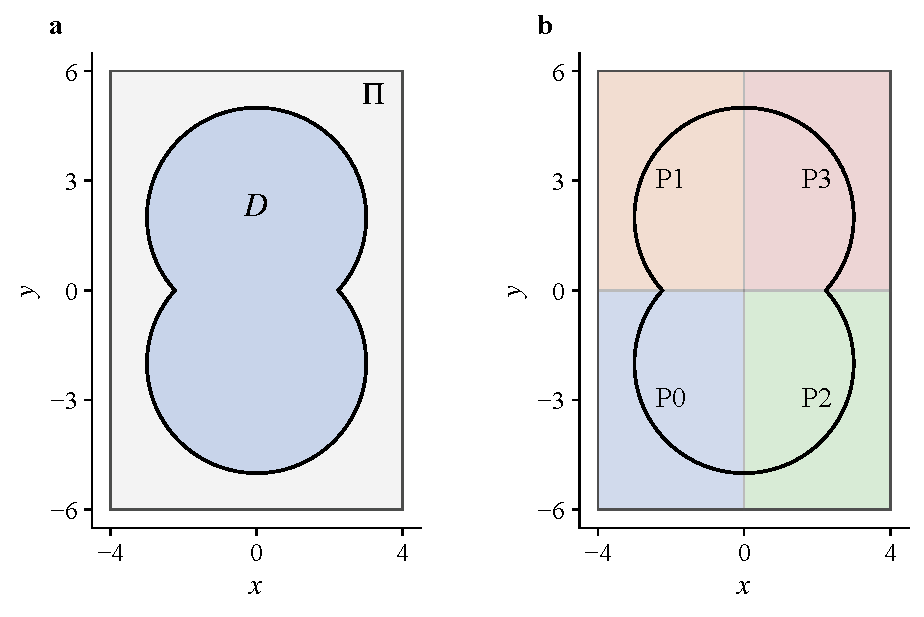
\includegraphics[width=0.94\linewidth]{figures/geometry.pdf}
    \caption{Расчётная геометрия: \textbf{a} область $D$ внутри прямоугольника $\Pi$; \textbf{b} пример разбиения $\Pi$ между четырьмя MPI-процессами. Цвет обозначает принадлежность геометрической подобласти процессу; граница исходной области показана чёрной линией.}
    \label{fig:geometry}
\end{figure}

Программа вычисляет приближённые значения $u$ в узлах сетки.
Для одной и той же схемы реализованы последовательный алгоритм, версия OpenMP, версия MPI и гибридная версия MPI+OpenMP.
Сравниваются полученные решения, число итераций и время вычислений.

\section{Метод фиктивных областей}

Прямоугольная сетка позволяет использовать одинаковый шаблон вычислений во всех узлах.
Для учёта криволинейной границы за пределами $D$ в уравнение вводится штрафной член, который приближает решение к заданному продолжению граничной функции.
В качестве продолжения выбрана функция $g(x,y)=\sin(x+y)$.
Задача в прямоугольнике имеет вид
\begin{equation}
    -\Delta v+Q(x,y)(v-g)=F(x,y) \quad \text{в }\Pi,
    \qquad v=g \quad \text{на }\partial\Pi,
    \label{eq:penalty}
\end{equation}
где
\begin{equation}
    Q(x,y)=\begin{cases}0,&(x,y)\in D,\\ \varepsilon^{-2},&(x,y)\in\Pi\setminus D,\end{cases}
    \qquad
    F(x,y)=\begin{cases}1,&(x,y)\in D,\\0,&(x,y)\in\Pi\setminus D.\end{cases}
    \label{eq:coefficients}
\end{equation}
При малом $\varepsilon$ член $Q(v-g)$ ограничивает отклонение $v$ от $g$ в фиктивной области.
Внутри $D$ сохраняется исходное уравнение Пуассона.
Согласно условию задания, используется $\varepsilon=h^2$, где $h$ есть наибольший шаг сетки~\cite{assignment}.
Такой выбор параметра сам по себе не задаёт точность конечного сеточного решения.

\section{Разностная схема}

Пусть $M$ и $N$ обозначают числа интервалов по координатам $x$ и $y$.
Узлы прямоугольной сетки задаются формулами
\begin{equation}
    \begin{aligned}
        x_i & =-4+ih_x,\quad h_x=8/M,\quad 0\leq i\leq M;  \\
        y_j & =-6+jh_y,\quad h_y=12/N,\quad 0\leq j\leq N.
    \end{aligned}
\end{equation}
Полная сетка содержит $(M+1)(N+1)$ узлов.
Значения на внешней границе известны, поэтому число неизвестных равно $K=(M-1)(N-1)$.
Запись $M\times N$ обозначает числа интервалов по координатам.

\subsection{Коэффициенты около границы}

Для каждого внутреннего узла $(i,j)$ вводится ячейка
\begin{equation}
    \Pi_{ij}=[x_i-h_x/2,x_i+h_x/2]\times[y_j-h_y/2,y_j+h_y/2].
\end{equation}
Обозначим площадь пересечения этой ячейки с $D$ через $S_{ij}$.
Тогда $s_{ij}=S_{ij}/(h_xh_y)$ равно доле её площади внутри области.
Усреднение коэффициентов из~\eqref{eq:coefficients} даёт
\begin{equation}
    F_{ij}=s_{ij},\qquad Q_{ij}=\frac{1-s_{ij}}{\varepsilon^2}, \qquad \varepsilon=\max(h_x,h_y)^2.
    \label{eq:cellcoeff}
\end{equation}
В полностью внутренней ячейке $s_{ij}=1$, в полностью внешней $s_{ij}=0$.
Частично пересечённые ячейки учитывают положение границы без округления до ближайшего узла.

Площадь $S_{ij}$ вычисляется аналитическим интегрированием горизонтальных сечений.
При $y\geq0$ граница относится к кругу с центром $(0,2)$, при $y<0$ к кругу с центром $(0,-2)$.
Полуширина сечения равна $\sqrt{9-(|y|-2)^2}$ там, где подкоренное выражение неотрицательно.
Интервал интегрирования делится в точках $y=0$ и пересечения дуги с вертикальными сторонами ячейки.
На каждом участке используется первообразная
\begin{equation}
    \int\sqrt{9-t^2}\,dt
    =\frac{t\sqrt{9-t^2}+9\arcsin(t/3)}{2}.
\end{equation}
Геометрическое интегрирование не содержит дополнительного параметра дискретизации.

\subsection{Система линейных уравнений}

Вторая производная заменяется центральной разностью.
Для внутренних узлов, то есть $1\leq i\leq M-1$ и $1\leq j\leq N-1$, получается уравнение
\begin{equation}
    -\frac{v_{i+1,j}-2v_{ij}+v_{i-1,j}}{h_x^2}
    -\frac{v_{i,j+1}-2v_{ij}+v_{i,j-1}}{h_y^2}
    +Q_{ij}(v_{ij}-g_{ij})=F_{ij},
    \label{eq:stencil}
\end{equation}
где $g_{ij}=\sin(x_i+y_j)$.
Известные граничные значения переносятся в правую часть.
Матрица $\mat A\in\mathbb R^{K\times K}$ симметрична и положительно определена: к разностному оператору $-\Delta$ с условиями Дирихле добавляется неотрицательная диагональ $Q_{ij}$.
Её действие вычисляется по пятиузловому шаблону, без хранения полной матрицы.

На мелких сетках $\varepsilon^{-2}$ становится большим.
Чтобы избежать вычитания больших близких слагаемых $Q_{ij}v_{ij}$ и $Q_{ij}g_{ij}$, решается эквивалентная система для поправки $w_{ij}=v_{ij}-g_{ij}$:
\begin{equation}
    \mat A\vect w=\vect b,\qquad
    b_{ij}=F_{ij}-\lambda_h g_{ij},\qquad
    \lambda_h=\frac{4\sin^2(h_x/2)}{h_x^2}
    +\frac{4\sin^2(h_y/2)}{h_y^2}.
    \label{eq:shifted}
\end{equation}
Формула для $\lambda_h$ следует из применения центральных разностей к $\sin(x+y)$.
На внешней границе поправка равна нулю.
После решения восстанавливается $v_{ij}=w_{ij}+g_{ij}$; именно эти значения сохраняются как результат.
Жирные символы $\vect w,\vect b\in\mathbb R^K$ обозначают векторы внутренних узлов, упорядоченных по двум индексам сетки.

\section{Метод сопряжённых градиентов}

Симметрия и положительная определённость $\mat A$ позволяют использовать метод сопряжённых градиентов~\cite{cg}.
Диагональный предобуславливатель $\mat D$ уменьшает различие масштабов коэффициентов:
\begin{equation}
    D_{ij}=2/h_x^2+2/h_y^2+Q_{ij}.
\end{equation}
Здесь $D_{ij}$ обозначает диагональный коэффициент, соответствующий узлу $(i,j)$.
Вектор невязки $\vect r=\vect b-\mat A\vect w$ показывает, насколько текущее приближение удовлетворяет системе.
Вектор $\vect z=\mat D^{-1}\vect r$ получается делением каждого элемента невязки на соответствующий диагональный коэффициент.
Во всех скалярных произведениях используется сеточная мера:
\begin{equation}
    \inner{\vect a}{\vect b}=h_xh_y\sum_{i=1}^{M-1}\sum_{j=1}^{N-1}a_{ij}b_{ij},
    \qquad \normE{\vect a}=\sqrt{\inner{\vect a}{\vect a}}.
\end{equation}

Начальное приближение для поправки $\vect w^{(0)}=0$ соответствует $v^{(0)}=g$.
Вычисляются $\vect r^{(0)}=\vect b$, $\vect z^{(0)}=\mat D^{-1}\vect r^{(0)}$ и $\vect p^{(0)}=\vect z^{(0)}$.
На итерации $k=0,1,\ldots$ используются формулы
\begin{align}
    \alpha_k        & =\frac{\inner{\vect r^{(k)}}{\vect z^{(k)}}}
    {\inner{\mat A\vect p^{(k)}}{\vect p^{(k)}}},                  \\
    \vect w^{(k+1)} & =\vect w^{(k)}+\alpha_k\vect p^{(k)},\qquad
    \vect r^{(k+1)}=\vect r^{(k)}-\alpha_k\mat A\vect p^{(k)},     \\
    \vect z^{(k+1)} & =\mat D^{-1}\vect r^{(k+1)},\qquad
    \beta_k=\frac{\inner{\vect r^{(k+1)}}{\vect z^{(k+1)}}}
    {\inner{\vect r^{(k)}}{\vect z^{(k)}}},                        \\
    \vect p^{(k+1)} & =\vect z^{(k+1)}+\beta_k\vect p^{(k)}.
\end{align}
Вектор $\vect p^{(k)}$ задаёт направление изменения решения, а $\alpha_k$ величину шага вдоль него.
Итерации останавливаются при выполнении условия задания
\begin{equation}
    \normE{\vect w^{(k+1)}-\vect w^{(k)}}<\delta.
    \label{eq:stop}
\end{equation}
Для основных расчётов выбрано $\delta=10^{-8}$, а для проверки на известном решении $\delta=10^{-10}$.
Это порог изменения итерации, а не оценка ошибки исходной краевой задачи.
После остановки невязка повторно вычисляется непосредственно как $\vect b-\mat A\vect w$.

Дополнительно контролируется функционал
\begin{equation}
    J(\vect w)=\tfrac12\inner{\mat A\vect w}{\vect w}-\inner{\vect b}{\vect w} =-\tfrac12\inner{\vect b+\vect r}{\vect w}.
\end{equation}
Если его рост превышает $16\epsilon_{\rm mach}
    K\max(1,|J_k|,|J_{k+1}|)$, шаг откатывается и метод перезапускается с заново вычисленной невязкой.
Здесь $\epsilon_{\rm mach}$ обозначает машинную точность типа \code{double}; множитель $K$ учитывает накопление ошибок при суммировании.
Общее число итераций ограничено $K$, число допустимых перезапусков равно восьми.

\section{Параллельная реализация}

Все четыре программы написаны на C++17 и используют общий численный код.
Поэтому коэффициенты, начальное приближение и условие остановки во всех версиях совпадают.
Изменяется способ выполнения операций над локальными узлами и объединения результатов.

\subsection{OpenMP}

В версии OpenMP узлы одной прямоугольной сетки распределяются между потоками одного процесса.
Потоки работают с общей памятью и используют одни и те же массивы данных.
Двойные циклы для действия оператора, обновления векторов и вычисления скалярных произведений используют \code{parallel for collapse(2)} со статическим распределением итераций.
Суммы и максимумы вычисляются через \code{reduction}~\cite{omp}.
Каждый поток обновляет собственный набор элементов, поэтому одновременная запись в один узел не требуется.
Порядок сложения в редукции может отличаться от последовательного; побитовое совпадение результатов не предполагается.

\subsection{MPI}

MPI (Message Passing Interface) обеспечивает обмен сообщениями между процессами с раздельной памятью.
Каждый процесс хранит свою часть сетки.
MPI-процессы образуют прямоугольную решётку $P_x\times P_y$, где $P_xP_y=P$ и $P$ есть общее число процессов.
При выборе её размеров перебираются делители $P$.
Числа интервалов каждой координаты распределяются с остатком, поэтому размеры геометрических подобластей различаются не более чем на один интервал.
Среди допустимых разбиений выбирается ближайшее к квадрату по числу узлов.

Ограничение задания на отношение сторон применяется к узлам геометрической подобласти, включая общие интерфейсы.
Если в ней $m_x$ и $m_y$ интервалов, проверяется условие
\begin{equation}
    \frac12\leq\frac{m_x+1}{m_y+1}\leq2.
\end{equation}
При этом каждое внутреннее неизвестное имеет ровно одного владельца.
Например, при разбиении сетки $80\times80$ между двумя процессами геометрические подобласти имеют по $41\times81$ узлу с учётом общей границы.
Число принадлежащих процессу внутренних строк равно $39$ или $40$, поскольку всего таких строк $79$.

Для действия пятиузлового шаблона необходимы значения соседей за границей локального массива.
Они хранятся в дополнительном слое и обновляются перед каждым умножением на $\mat A$.
Обмен реализован четырьмя вызовами \code{MPI\_Sendrecv}; столбцы передаются с помощью производного типа данных~\cite{mpi}.
На обычной итерации выполняются два глобальных суммирования через \code{MPI\_Allreduce}: одно для шага $\alpha_k$, второе одновременно для нескольких скалярных величин после обновления решения.
Физические граничные узлы поправки остаются нулевыми.

\subsection{MPI+OpenMP}

Гибридная версия сохраняет MPI-разбиение и распараллеливает локальные циклы каждого процесса средствами OpenMP.
Число потоков задаётся одинаковым для всех процессов.
Все вызовы MPI выполняются главным потоком после окончания соответствующей параллельной области, что соответствует уровню \code{MPI\_THREAD\_FUNNELED}~\cite{mpi}.
Во время MPI-обмена остальные потоки процесса не выполняют локальные циклы решателя.

\section{Результаты расчётов}

\subsection{Вычислительная среда}

Расчёты выполнены 9 ноября 2026 года на IBM Polus.
Планировщик LSF выделил два вычислительных узла в исключительное пользование на время серии.
Каждый узел содержит два процессора POWER8NVL, по десять физических ядер в каждом.
Одно ядро поддерживает восемь аппаратных потоков, поэтому операционная система видит 160 логических процессоров на узел.
Аппаратные потоки одного ядра разделяют его вычислительные ресурсы.

Все четыре версии собраны GCC 7.3.1 из Advance Toolchain 11.0 с параметрами \code{-std=c++17 -O3 -DNDEBUG -mcpu=power8}.
Использованы Spectrum MPI 10.1.0 и библиотека OpenMP \code{libgomp} из той же поставки GCC.
Порог остановки основных расчётов равен $\delta=10^{-8}$.

Последовательная версия привязана к одному логическому процессору.
В конфигурациях OpenMP до 16 потоков каждый поток занимает отдельное физическое ядро.
Конфигурация с 32 потоками использует 16 физических ядер, по два аппаратных потока на ядро (SMT2).
Ядра выбираются поочерёдно из двух процессорных сокетов.
Динамическое изменение числа потоков отключено.

В MPI каждому процессу выделено отдельное ядро, а в гибридной версии каждому потоку процесса выделено своё ядро.
MPI с 32 процессами размещается по 16 процессов на двух узлах.
Гибридная конфигурация $4\times8$ использует по два процесса с восемью потоками на каждом узле.
Остальные конфигурации выполняются на одном узле.
Число процессов и потоков, имена узлов и назначенные логические процессоры проверены для каждого запуска.

\subsection{Протокол измерений}

Выполнены оба набора конфигураций из задания: основной набор на малых сетках и полный набор приложения на сетках $400\times600$ и $800\times1200$~\cite{assignment}.
С учётом последовательных базовых расчётов серия содержит 37 конфигураций.
Перед измерениями каждая из них запускалась один раз для прогрева.
Для малых сеток проведено семь измерительных повторов, для крупных три.
Порядок конфигураций перемешивался с начальным значением генератора $14$.
Всего получено 155 измерений времени; прогревы и отдельный запуск для сохранения поля решения в статистику не входят.

Время $T$ измеряется внутри программы и включает выделение и инициализацию рабочих векторов, итерации метода сопряжённых градиентов, MPI-обмены и редукции.
Подготовка геометрии, запуск процессов, финальная проверка невязки и запись CSV выполняются вне измеряемого участка.
Для MPI и гибридной версии берётся максимум времени по процессам.
В таблицах приведены медиана и диапазон от минимального до максимального времени; все повторы сохранены, включая выбросы.

Ускорение вычисляется относительно отдельной последовательной программы на той же сетке:
\begin{equation}
    S(P,T_{\rm th})=\frac{T_{\rm seq}}{T_{P,T_{\rm th}}}.
    \label{eq:speedup}
\end{equation}
Здесь $P$ обозначает число процессов, $T_{\rm th}$ число потоков в процессе, а времена в правой части являются медианами повторов.
Значение $S<1$ соответствует замедлению относительно последовательной версии.
На графиках отрезки разброса ограничены величинами $T_{\rm seq,min}/T_{\rm par,max}$ и $T_{\rm seq,max}/T_{\rm par,min}$.
Они показывают диапазон отношений наблюдавшихся времён и не являются доверительными интервалами.

\FloatBarrier
\subsection{Последовательное решение}

Число итераций растёт при сгущении сетки (табл.~\ref{tab:seq}).
На каждой сетке оно одинаково у всех четырёх реализаций.
Все основные запуски завершились по критерию~\eqref{eq:stop} без перезапуска метода.
Невязка вычислена после остановки по системе для поправки~\eqref{eq:shifted}.
Её норма увеличивается при сгущении сетки: выбранный критерий ограничивает изменение приближения между итерациями и не задаёт фиксированной нормы невязки.

\begin{table}[H]
    \PaperTableStyle
    \begin{threeparttable}
        \caption{Последовательные расчёты на Polus}
        \label{tab:seq}
        \begin{tabular*}{\linewidth}{@{\extracolsep{\fill}}rrrrr@{}}
            \toprule
            \textbf{Сетка} & \textbf{Итер.} & \textbf{$T$, с} & \textbf{Диапазон, с} & \textbf{$\normE{\vect r}$}\\
            \midrule
            \DataInput{sequential_rows}
            \bottomrule
        \end{tabular*}
        \begin{tablenotes}[flushleft]\PaperTableNotesStyle
            \item[] Семь повторов на малых сетках и три на крупных; $\vect r=\vect b-\mat A\vect w$. Приведена наибольшая норма невязки среди повторов.
        \end{tablenotes}
    \end{threeparttable}
\end{table}

Решение на сетке $800\times1200$ показано на рис.~\ref{fig:solution}.
Эта сетка содержит $962001$ узел, из них $958001$ внутренних неизвестных.
Внутри $D$ значения приближения лежат примерно от $-1.000$ до $3.195$.
На цветовой карте фиктивная область скрыта.
Сечение при $x=0$ показывает изменение решения внутри области относительно продолжения граничной функции $g$.
Функция $g$ используется в постановке штрафной задачи; точное решение исходной задачи неизвестно.

\begin{figure}[ht]
    \centering
    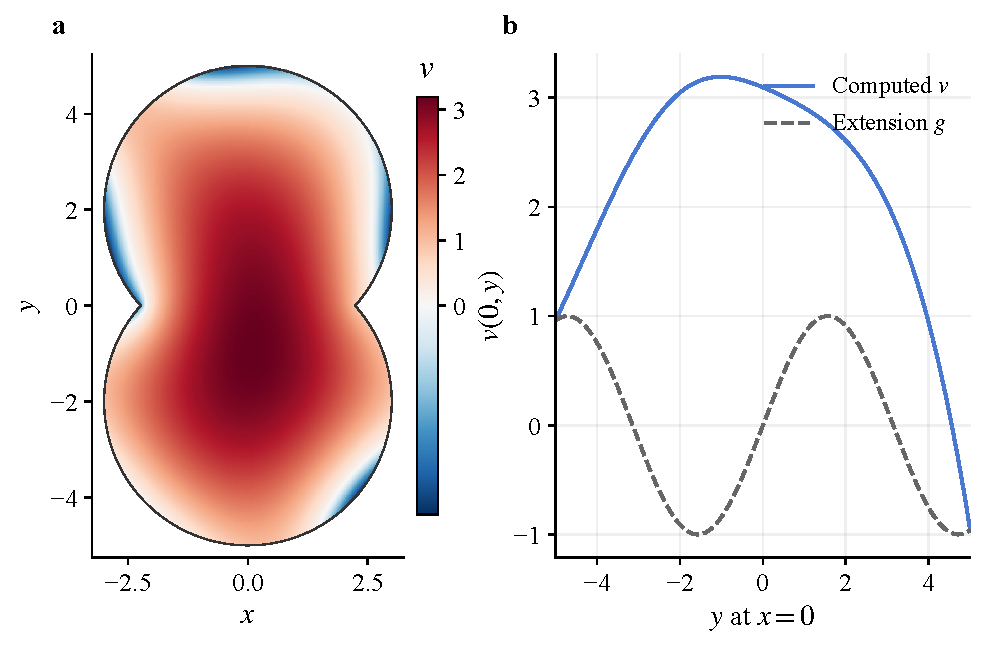
\includegraphics[width=\linewidth]{figures/solution.pdf}
    \caption{Решение на сетке $800\times1200$, полученное на Polus при $\varepsilon=h^2$ и $\delta=10^{-8}$: \textbf{a} значения $v$ внутри $D$; \textbf{b} сечение $v(0,y)$ и функция $g(0,y)=\sin y$. Последняя задаёт продолжение граничных данных, с которым сравнивается форма сечения.}
    \label{fig:solution}
\end{figure}

\FloatBarrier
\subsection{Проверка точности}

Для проверки численного метода решена вспомогательная задача с известным решением $v_*(x,y)=\sin(x+y)$.
В ней правая часть уравнения~\eqref{eq:penalty} заменена на $F_*(x,y)=2\sin(x+y)$ во всём прямоугольнике; коэффициент $Q$ и граничные условия сохранены.
Поскольку $-\Delta v_*=2v_*$ и $v_*-g=0$, эта функция точно удовлетворяет вспомогательной дифференциальной задаче при любом $\varepsilon$.
Проверяется ошибка
\begin{equation}
    E_h=\max_{1\leq i<M,\,1\leq j<N}|v_{ij}-v_*(x_i,y_j)|, \qquad p_h=\log_2\frac{E_{2h}}{E_h}.
\end{equation}
Величина $p_h$ оценивает наблюдаемый порядок уменьшения ошибки при двукратном сгущении сетки.

\begin{table}[H]
    \PaperTableStyle
    \begin{threeparttable}
        \caption{Проверка на известном решении}
        \label{tab:accuracy}
        \begin{tabular*}{\linewidth}{@{\extracolsep{\fill}}rrrr@{}}
            \toprule
            \textbf{Сетка} & \textbf{$h$} & \textbf{$E_h$} & \textbf{$p_h$}\\
            \midrule
            \DataInput{accuracy_rows}
            \bottomrule
        \end{tabular*}
        \begin{tablenotes}[flushleft]\PaperTableNotesStyle
            \item[] Проверка выполнена на Polus при $\delta=10^{-10}$. Порядок для первой строки не определяется.
        \end{tablenotes}
    \end{threeparttable}
\end{table}

Ошибки уменьшаются примерно в четыре раза при двукратном уменьшении шага.
График на рис.~\ref{fig:convergence} согласуется с зависимостью $E_h\sim h^2$ для выбранной гладкой тестовой функции.
Проверка подтверждает согласованность разностного оператора, граничных условий и решателя.
Порядок точности для исходной задачи с разрывной правой частью и приближённым условием на криволинейной границе отдельно не исследовался.

\begin{figure}[ht]
    \centering
    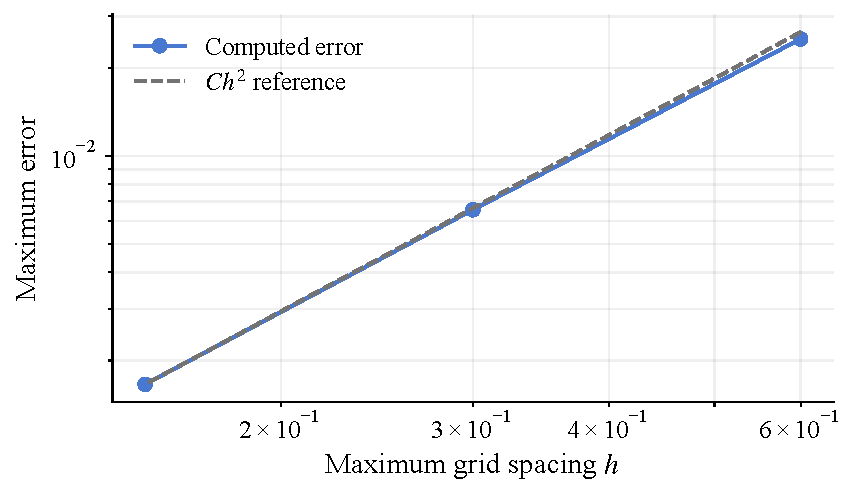
\includegraphics[width=0.82\linewidth]{figures/convergence.pdf}
    \caption{Максимальная ошибка для точного решения $v_* = \sin(x+y)$ на трёх сетках. Пунктирная линия пропорциональна $h^2$ и нормирована по ошибке на самой мелкой сетке. Обе оси логарифмические.}
    \label{fig:convergence}
\end{figure}

На сетке $6\times8$ результат сравнивался с независимым плотным решением системы методом исключения Гаусса.
В этой проверке площади ячеек получены численным интегрированием горизонтальных сечений.
При $\delta=10^{-10}$ максимальное различие составило $1.27\cdot10^{-7}$.
На сетках $23\times31$ и $80\times80$ решения последовательной и параллельных версий совпали с максимальным различием менее $8\cdot10^{-15}$ при том же пороге.
Первая сетка дополнительно проверяет неравномерное MPI-разбиение.

\FloatBarrier
\subsection{Малая сетка}

На сетке $80\times80$ все версии выполнили $193$ итерации для $6241$ неизвестного (табл.~\ref{tab:omp}, \ref{tab:mpi}, \ref{tab:hybrid}).
При сравнении используется медиана последовательного времени $16.420$ мс.

\begin{table}[H]
    \PaperTableStyle
    \begin{threeparttable}
        \caption{OpenMP на сетке $80\times80$}
        \label{tab:omp}
        \begin{tabular*}{\linewidth}{@{\extracolsep{\fill}}rrrrr@{}}
            \toprule
            \textbf{Потоки} & \textbf{Итерации} & \textbf{$T$, мс} & \textbf{Диапазон, мс} & \textbf{$S$}\\
            \midrule
            \DataInput{omp_rows}
            \bottomrule
        \end{tabular*}
        \begin{tablenotes}[flushleft]\PaperTableNotesStyle
            \item[] Семь повторов на одном узле. Каждый поток занимает отдельное физическое ядро.
        \end{tablenotes}
    \end{threeparttable}
\end{table}

\begin{table}[H]
    \PaperTableStyle
    \begin{threeparttable}
        \caption{MPI на сетке $80\times80$}
        \label{tab:mpi}
        \begin{tabular*}{\linewidth}{@{\extracolsep{\fill}}rrrrr@{}}
            \toprule
            \textbf{Процессы} & \textbf{Итерации} & \textbf{$T$, мс} & \textbf{Диапазон, мс} & \textbf{$S$}\\
            \midrule
            \DataInput{mpi_rows}
            \bottomrule
        \end{tabular*}
        \begin{tablenotes}[flushleft]\PaperTableNotesStyle
            \item[] Семь повторов; все процессы работают на одном узле и используют отдельные физические ядра.
        \end{tablenotes}
    \end{threeparttable}
\end{table}

\begin{table}[H]
    \PaperTableStyle
    \begin{threeparttable}
        \caption{MPI+OpenMP на сетке $80\times80$}
        \label{tab:hybrid}
        \begin{tabular*}{\linewidth}{@{\extracolsep{\fill}}rrrrrr@{}}
            \toprule
            \textbf{$P$} & \textbf{$T_{\rm th}$} & \textbf{Итерации} & \textbf{$T$, мс} & \textbf{Диапазон, мс} & \textbf{$S$}\\
            \midrule
            \DataInput{hybrid_rows}
            \bottomrule
        \end{tabular*}
        \begin{tablenotes}[flushleft]\PaperTableNotesStyle
            \item[] Семь повторов на одном узле. $P$ обозначает число процессов, $T_{\rm th}$ число потоков в процессе.
        \end{tablenotes}
    \end{threeparttable}
\end{table}

Наибольшее ускорение малой задачи получено для MPI с четырьмя процессами: $S=2.253$.
OpenMP с четырьмя потоками даёт $S=1.825$, а переход к 16 потокам снижает медианное ускорение до $1.389$.
У этой конфигурации также наблюдается выброс времени до $60.440$ мс при медиане $11.818$ мс.
Гибридная версия на двух процессах по четыре потока достигает $S=1.801$.
Сравнение конфигураций показано на рис.~\ref{fig:small-speedup}.

\begin{figure}[ht]
    \centering
    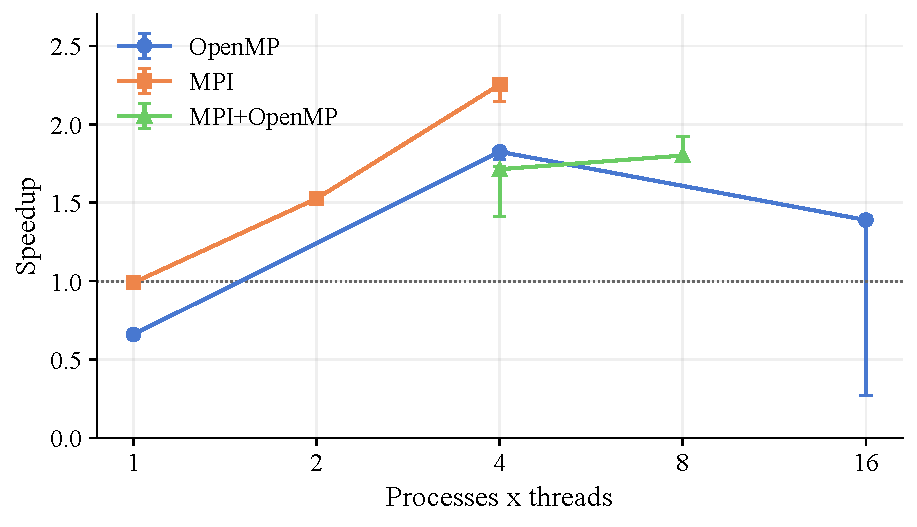
\includegraphics[width=0.90\linewidth]{figures/speedup_small.pdf}
    \caption{Ускорение на сетке $80\times80$. По горизонтали отложено произведение числа процессов и потоков; для гибрида $T_{\rm th}=4$. Маркеры показывают отношение медиан, отрезки показывают диапазон по повторам, определённый после формулы~\eqref{eq:speedup}. Пунктир соответствует $S=1$.}
    \label{fig:small-speedup}
\end{figure}

На обычной итерации программа выполняет четыре параллельные области OpenMP, а MPI-версия обменивается граничными слоями и вычисляет глобальные суммы.
Затраты на эти операции входят в измеренное время.
Их отдельный вклад на малой сетке не измерялся.

\FloatBarrier
\subsection{Крупные сетки}

Полные результаты приложения приведены в табл.~\ref{tab:large-omp}, \ref{tab:large-mpi} и~\ref{tab:large-hybrid}.
На сетке $400\times600$ все версии выполняют $1076$ итераций, на $800\times1200$ выполняют $2100$.
Последовательные базовые времена равны $3.473133$ и $28.095409$ с соответственно.

\begin{table}[H]
    \PaperTableStyle
    \begin{threeparttable}
        \caption{OpenMP на крупных сетках}
        \label{tab:large-omp}
        \begin{tabular*}{\linewidth}{@{\extracolsep{\fill}}rrrrr@{}}
            \toprule
            \textbf{Потоки} & \textbf{Итерации} & \textbf{$T$, с} & \textbf{Диапазон, с} & \textbf{$S$}\\
            \midrule
            \DataInput{large_omp_rows}
            \bottomrule
        \end{tabular*}
        \begin{tablenotes}[flushleft]\PaperTableNotesStyle
            \item[] Три повтора на одном узле. До 16 потоков используются отдельные физические ядра; 32 потока работают на 16 ядрах в режиме SMT2.
        \end{tablenotes}
    \end{threeparttable}
\end{table}

\begin{table}[H]
    \PaperTableStyle
    \begin{threeparttable}
        \caption{MPI на крупных сетках}
        \label{tab:large-mpi}
        \begin{tabular*}{\linewidth}{@{\extracolsep{\fill}}rrrrrr@{}}
            \toprule
            \textbf{Процессы} & \textbf{Итер.} & \textbf{Узлы} & \textbf{$T$, с} & \textbf{Диапазон, с} & \textbf{$S$}\\
            \midrule
            \DataInput{large_mpi_rows}
            \bottomrule
        \end{tabular*}
        \begin{tablenotes}[flushleft]\PaperTableNotesStyle
            \item[] Три повтора. Каждому процессу выделено отдельное физическое ядро. Конфигурация с 32 процессами использует по 16 ядер двух узлов.
        \end{tablenotes}
    \end{threeparttable}
\end{table}

\begin{table}[H]
    \PaperTableStyle
    \begin{threeparttable}
        \caption{MPI+OpenMP на крупных сетках}
        \label{tab:large-hybrid}
        \begin{tabular*}{\linewidth}{@{\extracolsep{\fill}}rrrrrrr@{}}
            \toprule
            \textbf{$P$} & \textbf{$T_{\rm th}$} & \textbf{Итер.} & \textbf{Узлы} & \textbf{$T$, с} & \textbf{Диапазон, с} & \textbf{$S$}\\
            \midrule
            \DataInput{large_hybrid_rows}
            \bottomrule
        \end{tabular*}
        \begin{tablenotes}[flushleft]\PaperTableNotesStyle
            \item[] Три повтора. Каждому потоку выделено отдельное физическое ядро; в конфигурации $4\times8$ по два процесса размещены на каждом из двух узлов.
        \end{tablenotes}
    \end{threeparttable}
\end{table}

На сетке $400\times600$ лучшие ускорения в проверенных конфигурациях равны $9.140$ для OpenMP, $13.995$ для MPI и $7.565$ для гибрида.
Эти значения получены при использовании 16 физических ядер одного узла.
На сетке $800\times1200$ наибольшее ускорение всей серии, $25.779$, даёт MPI с 32 процессами на двух узлах.
Гибрид $4\times8$ на тех же 32 физических ядрах достигает $S=15.933$.
OpenMP с 32 аппаратными потоками на 16 ядрах одного узла даёт $S=12.779$.
Одинаковое число программных исполнителей в этих трёх конфигурациях соответствует разным аппаратным ресурсам.

Ускорение MPI зависит от конфигурации немонотонно.
На сетке $400\times600$ переход от двух процессов к четырём увеличивает медиану времени с $1.772$ до $4.312$ с; при восьми процессах время снижается до $0.457$ с.
На сетке $800\times1200$ переход от восьми процессов к 16 увеличивает время с $3.521$ до $8.443$ с.
Эти замедления наблюдаются во всех трёх повторах (рис.~\ref{fig:large-speedup}).

\subsection{Границы интерпретации}

Измерения выполнены в одной сессии выделения ресурсов Polus с фиксированными компилятором и схемой размещения.
Диапазоны времени для крупных задач характеризуют разброс трёх повторов внутри этой сессии.
Время обменов, редукций и локальных операций отдельно не измерялось, поэтому причины немонотонных замедлений MPI не установлены.

В конфигурациях MPI с 32 процессами и гибрида $4\times8$ переход к двум узлам сопровождается увеличением числа физических ядер.
Сравнение одного и двух узлов при одинаковом числе ядер не проводилось, поэтому влияние межузлового размещения отдельно не оценено.

\begin{figure}[p]
    \centering
    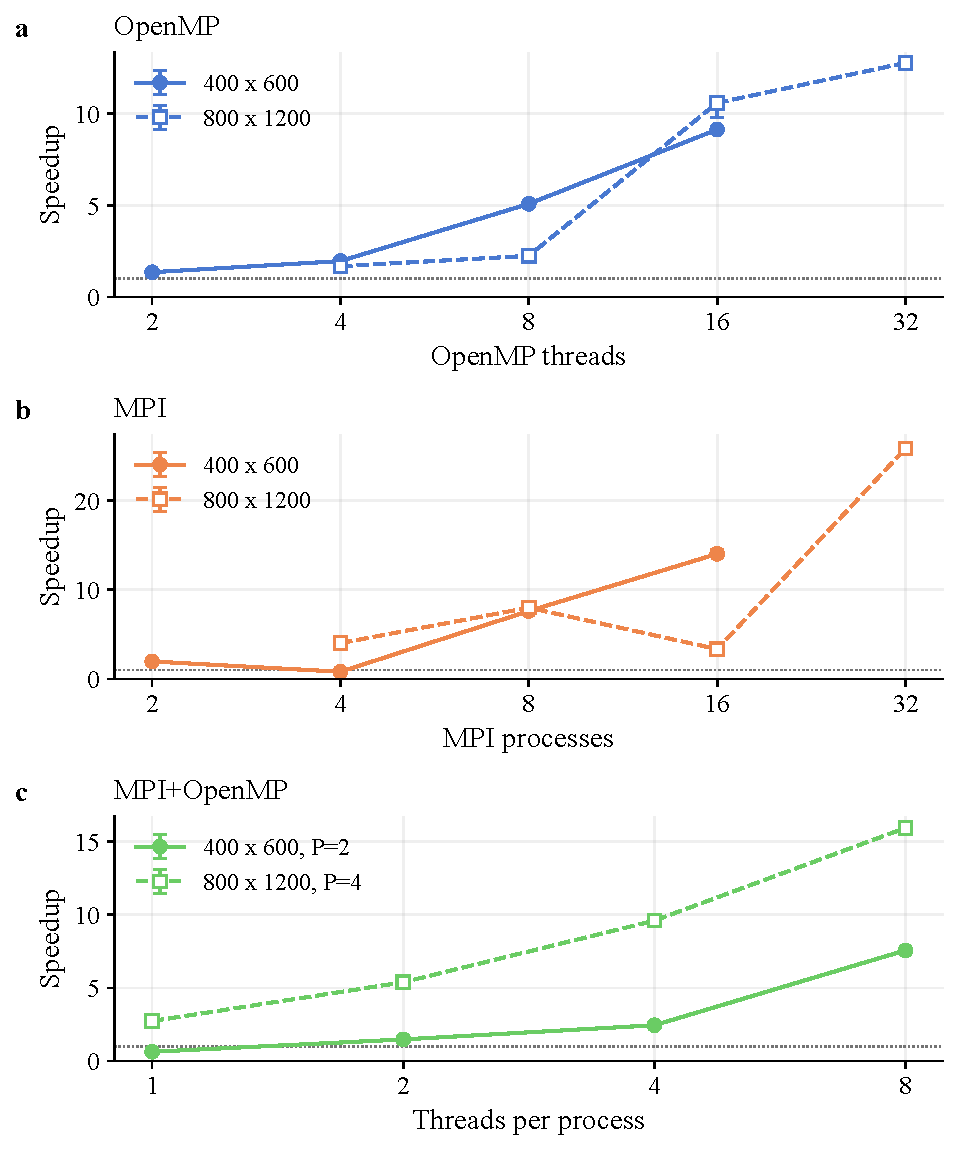
\includegraphics[width=\linewidth]{figures/speedup_large.pdf}
    \caption{Ускорение на крупных сетках: \textbf{a}
        OpenMP; \textbf{b} MPI; \textbf{c} MPI+OpenMP.
        Сплошная линия соответствует $400\times600$, штриховая линия соответствует $800\times1200$. Для гибрида число процессов фиксировано: $P=2$ на первой сетке и $P=4$ на второй. Отрезки показывают диапазон по повторам.
        OpenMP с 32 потоками использует SMT2 на одном узле; MPI с 32 процессами и гибрид $4\times8$ используют два узла.
    }
    \label{fig:large-speedup}
\end{figure}

\FloatBarrier

\clearpage
\section{Заключение}

Для области варианта 14 решена задача Дирихле для уравнения Пуассона методом фиктивных областей.
Коэффициенты разностной схемы учитывают долю площади каждой ячейки внутри области.
Система решается методом сопряжённых градиентов с диагональным предобуславливанием; замена неизвестной на поправку к $\sin(x+y)$ устраняет вычитание больших штрафных слагаемых.

Последовательная, OpenMP-, MPI- и гибридная реализации дают согласованные результаты.
Проверка с известным гладким решением показывает уменьшение ошибки примерно в четыре раза при двукратном сгущении сетки.
Для исходной задачи получено поле решения на сетке $800\times1200$.

На IBM Polus выполнены все 37 конфигураций основного набора и приложения, включая последовательные базовые расчёты.
На сетке $800\times1200$ MPI с 32 процессами на двух узлах сокращает медианное время с $28.095$ до $1.090$ с, что соответствует ускорению $25.779$.
Гибридная версия на 32 физических ядрах даёт ускорение $15.933$; OpenMP с 32 аппаратными потоками на 16 ядрах одного узла даёт $12.779$.

Для части MPI-конфигураций увеличение числа процессов приводит к повторяемому замедлению.
Причины замедлений в проведённых измерениях не установлены.
Полученные времена и ускорения относятся к зафиксированным условиям данной серии запусков.

\clearpage
\printbibliography[heading=bibintoc,title={Литература}]
\end{document}
